%% Overleaf			
%% Software Manual and Technical Document Template	
%% 									
%% This provides an example of a software manual created in Overleaf.

\documentclass{../ol-softwaremanual}

% Packages used in this example
\usepackage{graphicx}  % for including images
\usepackage{microtype} % for typographical enhancements
\usepackage{minted}    % for code listings
\usepackage{amsmath}   % for equations and mathematics
\setminted{style=friendly,fontsize=\small}
\renewcommand{\listoflistingscaption}{List of Code Listings}
\usepackage{hyperref}  % for hyperlinks
\usepackage[a4paper,top=4.2cm,bottom=4.2cm,left=3.5cm,right=3.5cm]{geometry} % for setting page size and margins

\usepackage[english, greek]{babel}



\usepackage{subfig}


% Custom macros used in this example document
\newcommand{\doclink}[2]{\href{#1}{#2}\footnote{\url{#1}}}
\newcommand{\cs}[1]{\texttt{\textbackslash #1}}

\renewcommand\thesubfigure{\roman{subfigure}}

\begin{document}
	
	
	\begin{titlepage}
		
		
		% Frontmatter data; appears on title page
		\title{\en Project Description \\}
		\version{0.4}
		\softwarelogo{
\includegraphics[scale=0.4]{../CarBazaar_logo.png}}
	\end{titlepage}
	
	
	\maketitle
	
	\newpage
	
	\center{\textbf{Μέλη Ομάδας}}
	
	\vspace{60pt}
	
	
	
	\begin{table}[htbp!]
		\begin{tabular}{llll}
			Μεμελετζόγλου Χαρίλαος & 1069364 & \en st1069364@ceid.upatras.gr  & \gr 4ο έτος \\ 
			\\ Λέκκας Γεώργιος      &      1067430    &   \en st1067430@ceid.upatras.gr  & \gr 4ο έτος \\
			\\ Γιαννουλάκης Ανδρέας        &   1067387       & \en st1067387@ceid.upatras.gr  & \gr 4ο έτος         \\
			\\ Κανελλόπουλος Ιωακείμ        &  1070914        &    \en st1070914@ceid.upatras.gr     & \gr 4ο έτος   \\ 
		\end{tabular}
	\end{table}
	
	\center{\textbf{Υπεύθυνοι Παρόντος Τεχνικού Κειμένου}}
	
	\vspace{20pt}
	
	\begin{table}[htbp!]
		\begin{tabular}{ll}
			Μεμελετζόγλου Χαρίλαος & \en Editor \\
			\\ Λέκκας Γεώργιος      &   \en  Editor \\
			\\ Γιαννουλάκης Ανδρέας & \en Peer Reviewer \\
			\\ Κανελλόπουλος Ιωακείμ & \en Peer Reviewer
		\end{tabular}
	\end{table}
	
	\center{\textbf{Αλλαγές στην έκδοση \en v0.4 \gr}}
	\vspace{10pt}
	
	Ανανεωμένες \en Mockup Screens \gr για τα \en Use Cases \gr :
	
	\begin{itemize}
		\item \en \#2: \gr Προγραμματισμός Ελέγχου Οχήματος
		\item \en \#4: \gr Αναζήτηση Κοντινών Αντιπροσωπειών
		\item \en \#5: \gr Σύγκριση Αυτοκινήτων
		\item \en \#7: \gr Προγραμματισμός \en Test Drive \gr
		\item \en \#9: \gr Αγορά Οχήματος
		\item \en \#10: \gr Αναζήτηση Οχήματος
		\item \en \#12: \gr Ανάρτηση Αγγελίας Πώλησης Ανταλλακτικού
		\item \en \#14: \gr Αγορά Ασφαλιστικού Πακέτου
	\end{itemize}
	

	\vspace{10pt}	
	
	\center{\textbf{Εργαλεία που χρησιμοποιήθηκαν}}
	
	\vspace{20pt}
	\flushleft
	
	Χρησιμοποιήθηκε το \en \doclink{https://www.overleaf.com/}{Overleaf} \gr και το \en \doclink{https://www.texstudio.org/}{TexStudio} \gr για την συγγραφή του \LaTeX\ κώδικα. \break
	
	Για την δημιουργία του λογότυπου, χρησιμοποιήθηκε το εργαλείο \en \doclink{https://www.adobe.com/express/create/logo}{Adobe Express} . \gr \break
	
	Για την δημιουργία των \en Mock-up Screens \gr, χρησιμοποιήθηκε το \en \doclink{https://moqups.com/}{Moqups} \gr . \break
	
	Η δημιουργία των \en UI \gr οθονών, γίνεται με την χρήστη του \en \doclink{https://doc.qt.io/qt-5/qtdesigner-manual.html}{QtDesigner} \gr, και του  \en \textbf{PyQt} cross-platform Qt Framework \gr. \break
	
	\en 	\doclink{https://github.com/st1069364/CarBazaar}{Link \gr του \en  repository \gr του \en Project \gr στο \en Github}. \gr
	
	\newpage
	
	\center{\textbf{Περιγραφή Έργου}} 
	
	\vspace{10pt}
	
	\flushleft
	
	Θεωρούμε πως μια μεγάλη πολυεθνική που δραστηριοποιείται στον χώρο των ασφαλειών για οχήματα, επιθυμεί να δημιουργήσει μια νέα πλατφόρμα, με όνομα  \en \textbf{\textit{CarBazaar}} \gr, στην οποία θα διεξάγονται αγοραπωλησίες αυτοκινήτων και ανταλλακτικών τους. Μέσω διαγωνισμού που διεξήχθη, η ομάδα μας ανέλαβε να αναπτύξει την εν λόγω εφαρμογή. \break
	
	Στην εφαρμογή συμμετέχουν 5 διαφορετικοί τύποι χρηστών :
	
	\begin{itemize}
		\item Ιδιώτες (απλοί χρήστες)
		\item Αντιπροσωπείες Αυτοκινήτων
		\item Ελεγκτές Οχημάτων
		\item Μεταφορείς Οχημάτων
		\item Η Ασφαλιστική Εταιρεία (ως διαχειριστής του συστήματος)
	\end{itemize}
	
	Στην πλατφόρμα, πωλούνται και μεταχειρισμένα αλλά και καινούρια αυτοκίνητα. Στην πρώτη περίπτωση, ο πωλητής μπορεί να είναι είτε ιδιώτης είτε μια αντιπροσωπεία, ενώ στην δεύτερη περίπτωση, ο πωλητής είναι αποκλειστικά και μόνο μια αντιπροσωπεία.  \break	
	
	Το σύστημα παρέχει στους χρήστες του, μια υπηρεσία εκτίμησης της αξίας ενός \textit{μεταχειρισμένου} οχήματος, προκειμένου να μην υπερκοστολογήσουν ένα όχημα που διαθέτουν προς πώληση, αλλά και να γνωρίζουν πως η τιμή του αυτοκινήτου που ενδιαφέρονται να αγοράσουν, δεν είναι υψηλότερη απ' ότι πρέπει. \break
	
	Επίσης, με βάση τις φωτογραφίες που έχουν αναρτηθεί στην αγγελία πώλησης ενός οχήματος, το σύστημα είναι σε θέση να κατασκευάσει ένα 3\en D \gr μοντέλο, του εσωτερικού αλλά και του εξωτερικού χώρου του οχήματος. \break
	
	Μέσω της εφαρμογής, οι εμπλεκόμενοι χρήστες όλων των ειδών, μπορούν να ανταλλάσσουν μηνύματα, για την ομαλή διεξαγωγή των συναλλαγών. \break
	
	Ακόμη, η εφαρμογή διαθέτει υπηρεσία σκαναρίσματος και ανάρτησης των απαραίτητων νομικών εγγράφων που απαιτούνται κατά την αγοραπωλησία ή ανταλλαγή, ενός οχήματος αλλά και υπολογισμού των μηνιαίων δόσεων, στην περίπτωση που η αγορά γίνει μέσω άτοκων δόσεων. \break
	
	Οι χρήστες, μπορούν να αναζητήσουν αυτοκίνητα είτε με βάση τον τίτλο του μοντέλου είτε με βάση την μάρκα, το έτος κυκλοφορίας κλπ, αλλά και να αποθηκεύσουν αυτοκίνητα της αρεσκείας τους σε μια \en wishlist \gr, επιτρέποντας, έτσι, στην εφαρμογή να τους προτείνει παρόμοια αυτοκίνητα στο μέλλον. Σε περίπτωση που προταθεί στον χρήστη κάποιο όχημα που δεν τον ενδιαφέρει, ο χρήστης θα μπορεί να ενημερώσει το σύστημα σχετικά με την λανθασμένη πρόταση, με σκοπό την βελτίωση του \en Recommender System \gr της πλατφόρμας \break 
	
	Ο χρήστης έχει την δυνατότητα δημιουργίας μιας αγγελίας πώλησης ενός οχήματος ή ανταλλακτικού, αλλά και προγραμματισμού ενός ραντεβού \en Test Drive \gr ή ελέγχου ενός αυτοκινήτου που ενδιαφέρεται να αγοράσει ή να αναρτήσει προς πώληση. \break
	
	Η εφαρμογή μέσω \en Push Notifications \gr, υπενθυμίζει στους χρήστες τα ραντεβού που έχουν προγραμματίσει (είτε για \en Test Drive \gr, είτε για έλεγχο του οχήματος), ενημερώνει για πιθανές αλλαγές στα ραντεβού τους και παρέχει πληροφορίες σχετικά με πληρωμές. Επίσης, ανάλογα και με την περιοχή του, ο χρήστης ειδοποιείται για την ανάρτηση αγγελιών αυτοκινήτων που ανήκουν στα ενδιαφέροντά του, με βάση τα αυτοκίνητα που έχει προσθέσει στην \en wishlist \gr του, αλλά και το ιστορικό των προηγούμενων αναζητήσεών του. \break
	
	Επιπροσθέτως, είναι δυνατή η σύγκριση αυτοκινήτων με βάση μια λίστα από κριτήρια καθορισμένα από τον χρήστη (όπως τιμή, κατανάλωση, κλπ), με σκοπό την επιλογή του οχήματος που ικανοποιεί τις ανάγκες του, αλλά και υπολογισμός των ασφαλίστρων και τελών κυκλοφορίας ενός οχήματος. \break
	
	Μια σημαντική λειτουργία της εφαρμογής, είναι η εύρεση αντιπροσωπειών που βρίσκονται κοντά στην τοποθεσία του χρήστη. \break
	
	Οι ιδιώτες και οι αντιπροσωπείες, ανάλογα με τις κριτικές που έχουν λάβει, τον αριθμό των αγγελιών και των πωλήσεων που έχουν ολοκληρώσει επιτυχώς αλλά και με βάση τον αριθμό των προβολών των αγγελιών τους, ανταμείβονται από το σύστημα, με πόντους. Ανάλογα με τους πόντους που έχει συλλέξει ο χρήστης ή η αντιπροσωπεία, οι αγγελίες του/της θα εμφανίζονται ψηλότερα στα αποτελέσματα αναζητήσεων άλλων χρηστών. Επίσης (μόνο στην περίπτωση του ιδιώτη χρήστη) οι πόντοι μπορούν να εξαργυρωθούν για την εξασφάλιση έκπτωσης σε ασφάλιστρα της ασφαλιστικής εταιρείας που θα διαχειρίζεται το σύστημα. \break
	
	Οι χρήστες έχουν την δυνατότητα να ενεργοποιήσουν την \en Premium \gr συνδρομή, με σκοπό την απόκρυψη διαφημίσεων αλλά και την παροχή Οδικής Βοήθειας από την ασφαλιστική εταιρεία. \break
	
	\red{Τέλος, οι χρήστες έχουν την δυνατότητα να συμμετάσχουν στο Πρόγραμμα Ανταλλαγής Οχημάτων, μέσω του οποίου μπορούν να πουλήσουν ένα όχημά τους σε μια αντιπροσωπεία. Η αντιπροσωπεία θα εκτιμήσει την αγοραστική αξία του οχήματος με βάση τα χαρακτηριστικά και την κατάστασή του και θα προσφέρει στον χρήστη είτε την αξία του οχήματος σε μετρητά είτε θα αφαιρέσει το ποσό αυτό, από την επόμενη αγορά οχήματος που θα κάνει ο χρήστης. }\break
	
	\vspace{5pt}
	
	Μια αντιπροσωπεία οχημάτων, μπορεί να καταχωρήσει στην πλατφόρμα τα καταστήματά της, την τοποθεσία τους, αλλά και τα οχήματα που υπάρχουν διαθέσιμα σε κάθε κατάστημα. \break 
	Όπως αναφέρθηκε παραπάνω, οι αντιπροσωπείες μπορούν να εξαργυρώσουν τους πόντους που έχουν συλλέξει προκειμένου να εμφανίζονται οι αγγελίες τους, υψηλότερα στα αποτελέσματα αναζήτησης των χρηστών. Επίσης, μπορούν να αγοράσουν την δυνατότητα να στέλνουν \en Push Notifications \gr στους χρήστες σχετικά με οχήματα που αναρτούν προς πώληση ή σχετικά με προσφορές περιορισμένου χρόνου, αλλά και να προωθούν τις σχετικές διαφημίσεις. \break
	
	Ακόμη, οι αντιπροσωπείες μπορούν να επεξεργάζονται την σελίδα του εταιρικού τους προφίλ αλλά και να βλέπουν και να σχολιάζουν κριτικές χρηστών.	 \break 
	
	\vspace{5pt}	
	
	Οι ελεγκτές μπορούν να μισθωθούν από τον χρήστη, με σκοπό τον έλεγχο της κατάστασης του οχήματος το οποίο ενδιαφέρεται να αγοράσει ο χρήστης ή του οχήματος που αναρτά προς πώληση. \break
	
	Ακόμη, μπορούν να αναρτούν αγγελίες και διαφημίσεις προκειμένου να ενημερώνουν τους χρήστες σχετικά με τις υπηρεσίες που προσφέρουν. \break
	
	Παρομοίως, και για τους μεταφορείς οι οποίοι μπορούν να μισθωθούν προκειμένου να μεταφέρουν ένα όχημα στην περιοχή του χρήστη. Κατά την αγορά μεταφοράς οχήματος, ο χρήστης μπορεί να επιλέξει ανάμεσα στην κανονική παράδοση και την \en express \gr παράδοση, στην οποία το όχημα θα βρίσκεται στην τοποθεσία του χρήστη, μέσα σε 24 ώρες.		\break
	
	
	Τέλος, οι υπάλληλοι της ασφαλιστικής εταιρείας, παρέχουν \en Live 24/7 Support \gr στους χρήστες, με σκοπό την επίλυση, είτε ζητημάτων που μπορούν να προκύψουν κατά την διεξαγωγή συναλλαγών είτε νομικών ζητημάτων. \break
	
	Επίσης, η ασφαλιστική εταιρεία, μπορεί να προωθεί και να δημιουργεί διαφημίσεις και \en Push Notifications \gr, σχετικά με ασφαλιστικά πακέτα, προσφορές αλλά και την κυκλοφορία ενός νέου μοντέλου αυτοκινήτου. \break
	
	Ακόμη, ένας υπάλληλος της εταιρείας, είναι σε θέση να ελέγχει τις αναφορές αγγελιών, και να αφαιρεί αγγελίες σε περίπτωση που η αναφορά είναι βάσιμη και η αγγελία παραβιάζει τους όρους χρήσης της πλατφόρμας. \break
	
	Επιπροσθέτως, η εταιρεία είναι σε θέση να βλέπει στατιστικά στοιχεία και να διεξάγει \en Real-Time Analysis \gr, με σκοπό την προβολή στοιχείων όπως ο αριθμός των ενεργών αγγελιών, ο συνολικός αλλά και ημερήσιος αριθμός πωλήσεων που έχουν διεξαχθεί μέσω της εφαρμογής, τα συνολικά και ημερήσια κέρδη, ο αριθμός των εγγεγραμμένων αλλά και ενεργών χρηστών. \break 
	
	Η ενημέρωση της Βάσης Δεδομένων με τα μοντέλα οχημάτων που κυκλοφορούν στην αγορά αποτελεί, επίσης, ευθύνη της διαχειριστικής εταιρείας. \break
	
	Μια ακόμη σημαντική λειτουργία της ασφαλιστικής εταιρείας, είναι η δημιουργία και διαχείριση των \en Loyalty Programs \gr. Συγκεκριμένα, η εταιρεία έχει ένα πλήρες ιστορικό των συναλλαγών και πωλήσεων που διεξάγονται μέσω της πλατφόρμας, το οποίο ανανεώνεται δυναμικά. Έτσι, είναι δυνατόν να εξαχθούν στοιχεία όπως οι προτιμήσεις κάθε χρήστη σε μάρκες αυτοκινήτων. Η εταιρεία μπορεί να προσφέρει στον χρήστη πόντους, που μπορεί να εξαργυρώσει στην επόμενη αγορά αυτοκινήτου της συγκεκριμένης μάρκας, με σκοπό την εξασφάλιση έκπτωσης. \break 
	
	
	
	\newpage
	
	\center{\en \textbf{Mockup Screens} } \gr
	
	
	
	\begin{figure}[htbp!]
		\centering
		\subfloat[\centering \en Login Screen]{{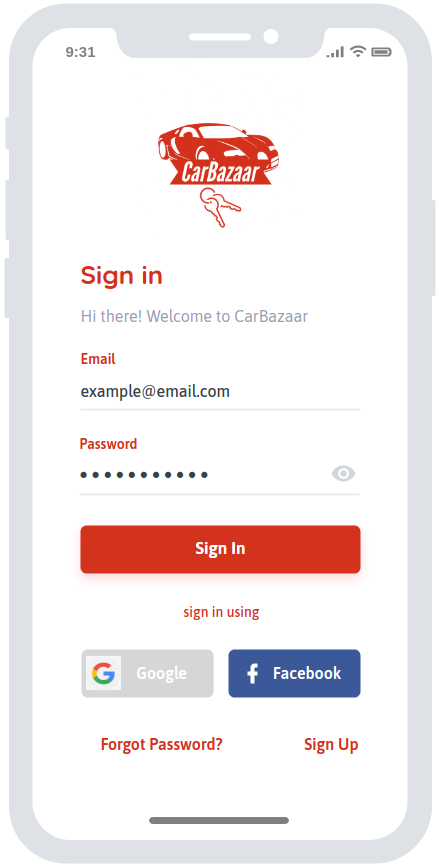
\includegraphics[scale=0.4]{img/mockups/login_screen.png} }}%
		\quad
		\subfloat[\centering \en Sign Up Screen]{{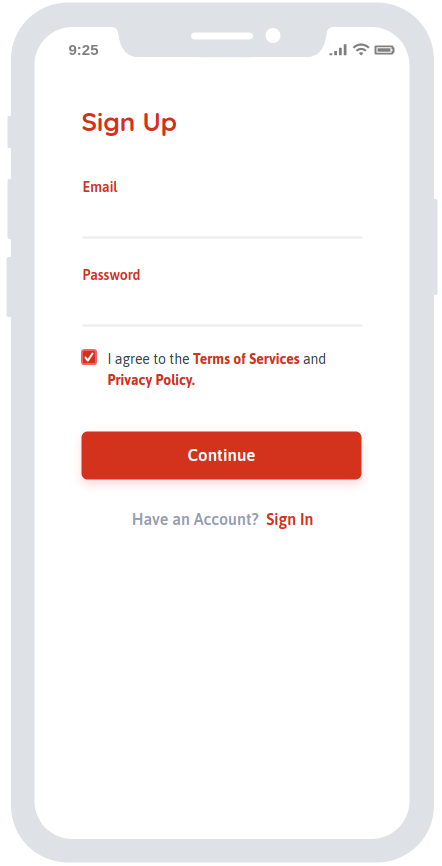
\includegraphics[scale=0.4]{img/mockups/signup_screen.png} }}%
		
		\subfloat[\centering \en User Menu]{{\includegraphics[scale=0.4]{img/mockups/user/user\_menu.png}}}%
	\end{figure}
	
	\newpage
	
	\centering { \textbf{ Αναζήτηση Ανταλλακτικού } } 
	
	\begin{figure}[htbp!]
		\subfloat[Βήμα 1 : Εισαγωγή στοιχείων Ανταλλακτικού]{{\includegraphics[scale=0.45]{img/mockups/user/spare\_parts\_search.png}}}%
		\qquad
		\subfloat[Βήμα 2 : Εμφάνιση λίστας Ανταλλακτικών]{{\includegraphics[scale=0.45]{img/mockups/user/spare\_part\_listing.png}}}%
		\qquad
		\subfloat[Βήμα 3 : Εμφάνιση συγκεκριμένου Ανταλλακτικού]{{\includegraphics[scale=0.45]{img/mockups/user/specific\_spare\_part.png}}}%
	\end{figure}
	
	\newpage
	
	\centering{ \textbf{Ανάρτηση Αγγελίας Πώλησης Οχήματος}}
	
	\begin{figure}[htbp!]
		\centering
		
		\subfloat[Βήμα 1 : Εισαγωγή τοποθεσίας και τίτλου αγγελίας]{{\includegraphics[scale=0.45]{img/mockups/post\_lst\_1.png}}}%
		\qquad
		\subfloat[Βήμα 2 : Εισαγωγή στοιχείων οχήματος]{{\includegraphics[scale=0.45]{img/mockups/post\_lst\_2.png}}}%
		\qquad
		\subfloat[Βήμα 3 : Εισαγωγή πιστοποιητικών εγγράφων κατάστασης οχήματος]{{\includegraphics[scale=0.45]{img/mockups/post\_lst\_3.png}}}%		
		\qquad
		\subfloat[Βήμα 4 : Τιμή Οχήματος]{{\includegraphics[scale=0.45]{img/mockups/post\_lst\_4.png}}}%
		\qquad
		\subfloat[Βήμα 5 : Εισαγωγή περιγραφής οχήματος]{{\includegraphics[scale=0.45]{img/mockups/post\_lst\_5.png}}}%
		\qquad
		\subfloat[Βήμα 6 : Προεπισκόπηση αγγελίας]{{\includegraphics[scale=0.45]{img/mockups/post\_lst\_6.png}}}%		
	\end{figure}	
	\newpage
	
	\centering { \textbf{ Προγραμματισμός \en Test Drive \gr } } 
	
	\begin{figure}[htbp!]
		\centering
		
		\subfloat[Βήμα 1 : Εισαγωγή κωδικού αγγελίας] {{\includegraphics[scale=0.45]{img/mockups/user/test\_drive\_1.png}}}%
		\qquad
		\subfloat[Βήμα 2 : Προγραμματισμός Ραντεβού \en Test Drive \gr] {{\includegraphics[scale=0.45]{img/mockups/user/test\_drive\_2.png}}}%
		\qquad
		\subfloat[Βήμα 3 : Επιβεβαίωση στοιχείων \en Test Drive \gr] {{\includegraphics[scale=0.45]{img/mockups/user/test\_drive\_3.png}}}%	
		\qquad	
		\subfloat[Εναλλακτική Ροή 1: Μήνυμα μη-διαθέσιμης ημερομηνίας] {{\includegraphics[scale=0.45]{img/mockups/user/test\_drive\_alt\_1.png}}}%
		\qquad
		\subfloat[Εναλλακτική Ροή 2: Μήνυμα μη-έγκυρου κωδικού αγγελίας] {{\includegraphics[scale=0.43]{img/mockups/user/test\_drive\_alt\_2.png}}}%
	\end{figure}
	
	\newpage	
	
	\centering{ \textbf{Αναζήτηση κοντινών αντιπροσωπειών}}
	
	\begin{figure}[htbp!]
		\centering
		
		\subfloat[Βήμα 1 : Εισαγωγή τοποθεσίας χρήστη] {{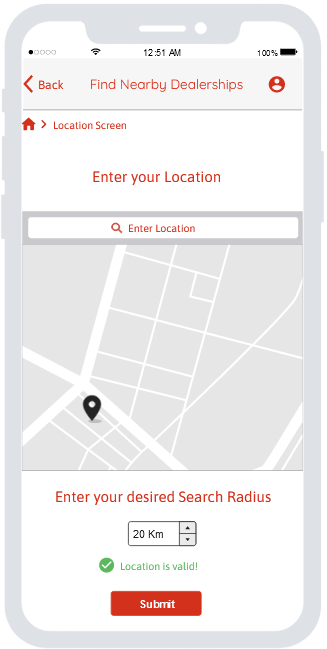
\includegraphics[scale=0.45]{img/mockups/user/dealership_loc.png}}}%
		\qquad
		\subfloat[Βήμα 2: Επιλογή Μαρκών Οχημάτων]{{\includegraphics[scale=0.45]{img/mockups/user/find\_dealership\_2.png}}}%
		\qquad
		\subfloat[Βήμα 3 : Εμφάνιση λίστας κοντινών αντιπροσωπειών] {{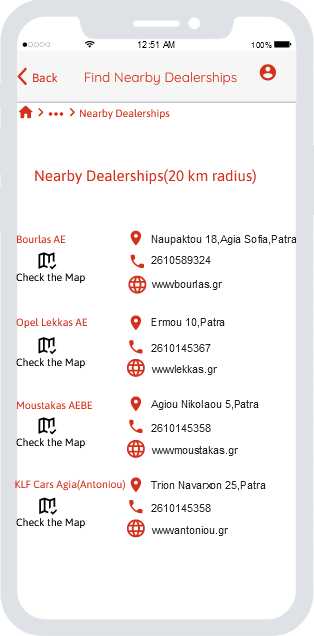
\includegraphics[scale=0.45]{img/mockups/user/dealership_list.png}}}%
		\qquad
		\subfloat[Βήμα 4 : Οθόνη συγκεκριμένης αντιπροσωπείας] {{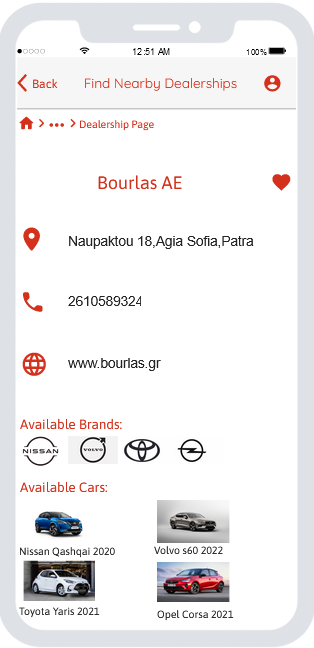
\includegraphics[scale=0.45]{img/mockups/user/specific_dlrship.png}}}%
	\end{figure}	
	
	\newpage	
	
	\centering{ \textbf{Προγραμματισμός Ελέγχου Οχήματος}}
	
	\begin{figure}[htbp!]
		\centering
		
		\subfloat[Βήμα 1 : Προγραμματισμός ραντεβού ελέγχου οχήματος] {{\includegraphics[scale=0.45]{img/mockups/user/car\_check\_1.png}}}%
		\qquad
		\subfloat[Βήμα 2 : Προτεινόμενος Ελεγκτής] {{\includegraphics[scale=0.47]{img/mockups/user/car\_check\_2.png}}}%
		\qquad
		\subfloat[Βήμα 3 : Λεπτομέρειες ραντεβού και πληρωμή] {{\includegraphics[scale=0.45]{img/mockups/user/car\_check\_3.png}}}%
		\qquad
		\subfloat[Βήμα 4 : Τιμή και διάρκεια Ελέγχου] {{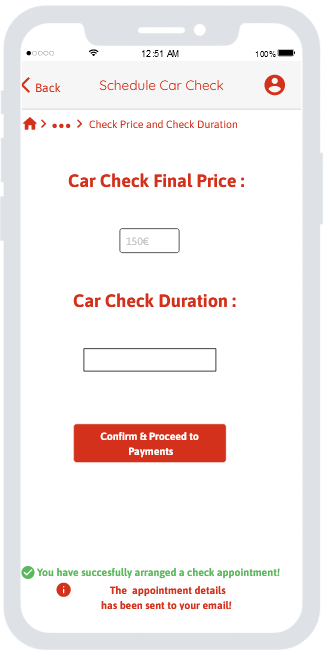
\includegraphics[scale=0.45]{img/mockups/user/car_check_4.png}}}%
		\qquad
		\subfloat[Εναλλακτική Ροή 2 : Ελεγκτής της αρεσκείας του χρήστη] {{\includegraphics[scale=0.47]{img/mockups/user/car\_check\_alt\_2.png}}}%
		\qquad
		
	\end{figure}
	
	
	\newpage
	
	
	\centering{ \textbf{Αναζήτηση Οχήματος}}
	
	\begin{figure}[htbp!]
		\centering			
		\subfloat[Βήμα 1 : Εισαγωγή στοιχείων οχήματος]{{\includegraphics[scale=0.45]{img/mockups/user/search\_1.png}}}%
		\qquad
		\subfloat[Βήμα 2 : Εισαγωγή στοιχείων τοποθεσίας, τύπου πωλητή και κριτηρίου ταξινόμησης ]{{\includegraphics[scale=0.45]{img/mockups/user/search\_2.png}}}%			
	\end{figure}
	
	
	\begin{figure}[htbp!]
		\centering			
		\subfloat[Βήμα 3 :  Αποτελέσματα αναζήτησης  ]{{\includegraphics[scale=0.45]{img/mockups/user/search\_3.png}}}%						
		\qquad					
		\subfloat[Βήμα 4 : Λεπτομέρειες αγγελίας]{{\includegraphics[scale=0.45]{img/mockups/user/search\_4.png}}}%				
	\end{figure}
	
	\newpage
	
	\centering{ \textbf{Σύγκριση Οχημάτων}}
	
	\begin{figure}[htbp!]
		\centering			
		\subfloat[Βήμα 1 : Εισαγωγή κωδικών αγγελιών και καθορισμός κριτηρίων σύγκρισης]{{\includegraphics[scale=0.45]{img/mockups/user/car\_comp\_1.png}}}%
		\qquad
		\subfloat[Βήμα 2 : Καθορισμός εύρους τιμών και κυρίαρχων κριτηρίων σύγκρισης]{{\includegraphics[scale=0.45]{img/mockups/user/car\_comp\_2.png}}}%		
		\qquad
		\subfloat[Βήμα 3 :  Αποτελέσματα σύγκρισης και επιλογής οχήματος]{{\includegraphics[scale=0.45]{img/mockups/user/car\_comp\_3.png}}}%
		\qquad
		\subfloat[Εναλλακτική Ροή 1 : Σύγκριση αυτοκινήτων από την \en Wishlist \gr και συχνά συγκρινόμενων αυτοκινήτων]{{\includegraphics[scale=0.45]{img/mockups/user/car\_comp\_alt\_1.png}}}%			
		\qquad			
		\subfloat[Εναλλακτική Ροή 2 : Προειδοποιητικό μήνυμα λόγω ίδιων κωδικών αγγελιών]{{\includegraphics[scale=0.45]{img/mockups/user/car\_comp\_alt\_2.png}}}%			
	\end{figure}
	
	\newpage
	
	\centering{ \textbf{Αγορά Οχήματος}}
	
	\begin{figure}[htbp!]
		\centering			
		\subfloat[Βήμα 1 : Εισαγωγή κωδικού ασφαλείας]{{\includegraphics[scale=0.47]{img/mockups/user/buy\_car\_1.png}}}%
		\qquad
		\subfloat[Βήμα 2 : Εισαγωγή κωδικού αγγελείας]{{\includegraphics[scale=0.47]{img/mockups/user/buy\_car\_2.png}}}%
		\qquad
		\subfloat[Βήμα 3 : Οικονομικές Επιλογές ]{{\includegraphics[scale=0.49]{img/mockups/user/buy\_car\_3.png}}}%
		\qquad		
		\subfloat[Βήμα 4 : Εισαγωγή Μηνιαίου μισθού και υπολογισμός μηνιαίας δόσης] {{\includegraphics[scale=0.47]{img/mockups/user/buy\_car\_4.png}}}%
		\qquad
		\subfloat[Βήμα 5 : Λεπτομέρειες Αγοράς]{{\includegraphics[scale=0.47]{img/mockups/user/buy\_car\_5.png}}}%	
	\end{figure}
	
	\newpage
	
	\centering{ \textbf{Επεξεργασία Αγγελίας}}
	
	\begin{figure}[htbp!]
		\centering			
		\subfloat[Βήμα 1 : Λίστα προυπάρχοντων αγγελιών]{{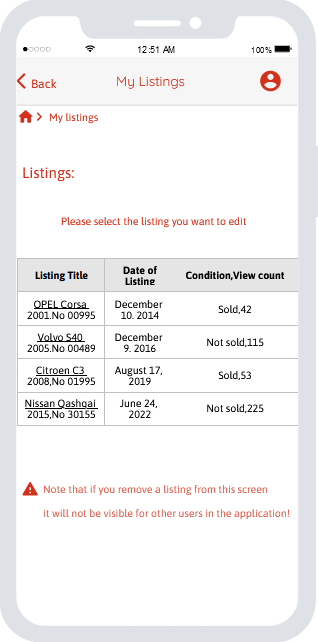
\includegraphics[scale=0.47]{img/mockups/user/edit_listings.png}}}%
		\qquad
		\subfloat[Βήμα 2 : Επεξεργασία αγγελίας] {{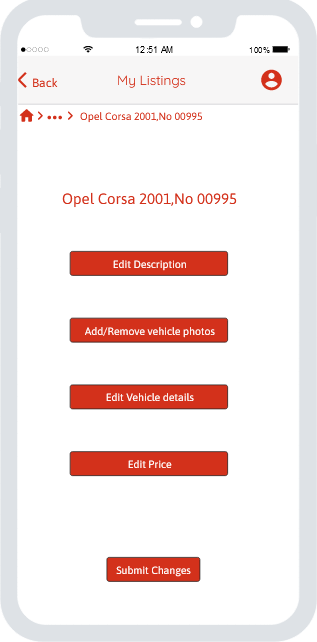
\includegraphics[scale=0.47]{img/mockups/user/submit_changes_lis.png}}}%
		
	\end{figure}
	\newpage
	
	\centering{ \textbf{Ανάρτηση Αγγελίας Πώλησης Ανταλλακτικού}}
	
	\begin{figure}[htbp!]
		\centering			
		\subfloat[Βήμα 1 : Εισαγωγή τοποθεσίας και τίτλου αγγελίας]{{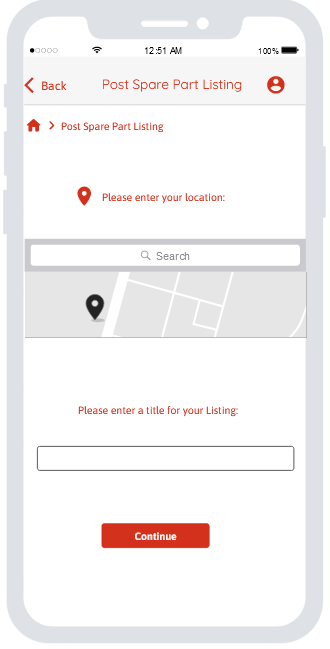
\includegraphics[scale=0.45]{img/mockups/user/spare_post_list_1.png}}}%
		\qquad
		\subfloat[Βήμα 2 : Λεπτομέρειες Ανταλλακτικού] {{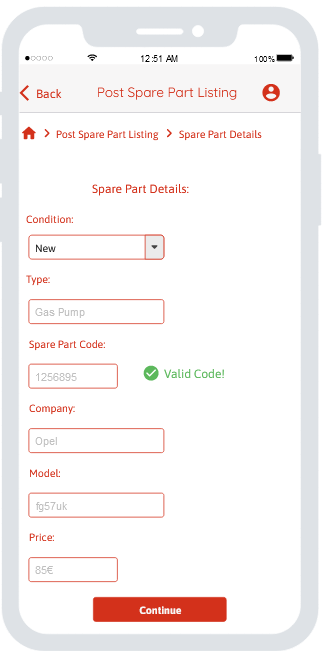
\includegraphics[scale=0.45]{img/mockups/user/spare_post_list_2.png}}}%
		\qquad
		\subfloat[Βήμα 3 : Εισαγωγή περιγραφής και εικόνων]{{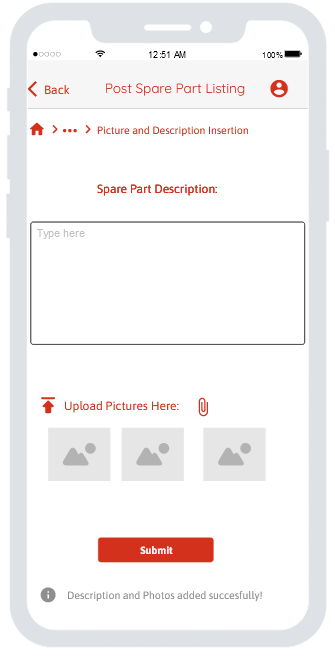
\includegraphics[scale=0.45]{img/mockups/user/spare_post_list_3.png}}}%
		\qquad
		\subfloat[Βήμα 4 : Προεπισκόπιση αγγελίας] {{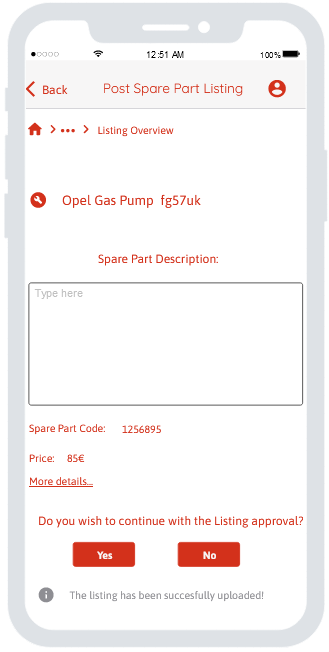
\includegraphics[scale=0.45]{img/mockups/user/spare_post_list_4.png}}}%
		\qquad
		\subfloat[Εναλλακτική Ροή 1 : Εμφάνιση προειδοποιητικού μηνύματος λόγω εισαγωγής λανθασμένου κωδικού ανταλλακτικού ]{{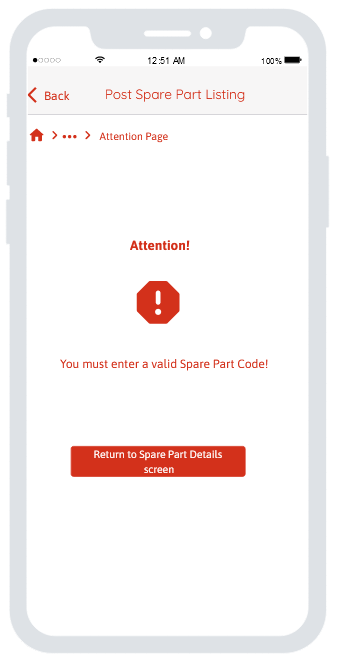
\includegraphics[scale=0.45]{img/mockups/user/alt_spare_post_list_1.png}}}%			
		\qquad			
		\subfloat[Εναλλακτική Ροή 2 : Προειδοποιητικό μήνυμα λόγω μη ύπαρξης εικόνων ή περιγραφής αγγελιών]{{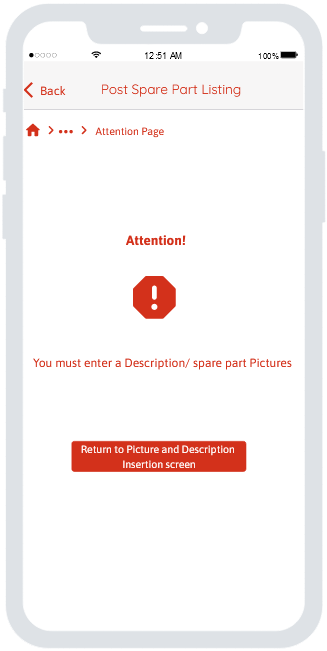
\includegraphics[scale=0.45]{img/mockups/user/alt_spare_post_list_2.png}}}%
	\end{figure}
	
	\newpage
	
	\centering{ \textbf{Αγορά Ασφαλιστικού Πακέτου}}
	
	\begin{figure}[htbp!]
		\centering			
		\subfloat[Βήμα 1 : Εισαγωγή κωδικού συναλλαγής]{{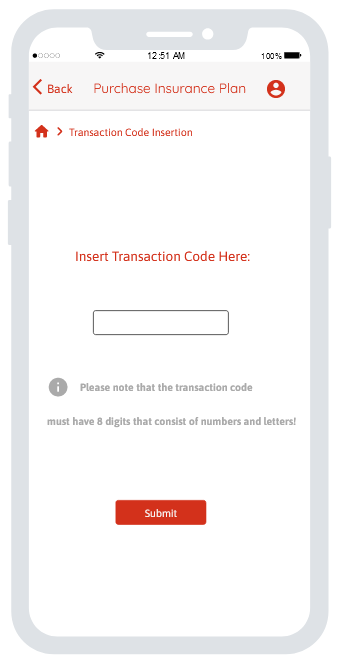
\includegraphics[scale=0.47]{img/mockups/user/ins_plan_1.png}}}%
		\qquad
		\subfloat[Βήμα 2 : Επιλογή Ασφαλιστικού Πακέτου] {{\includegraphics[scale=0.47]{img/mockups/user/ins_plan_2.png}}}%
		\qquad
		\subfloat[Βήμα 3 : Εισαγωγή τιμής και πληρωμή]{{\includegraphics[scale=0.47]{img/mockups/user/ins_plan_3.png}}}%
		\qquad
		\subfloat[Εναλλακτική Ροή 1 : Προειδοποιητική οθόνη λόγω λανθασμένου κωδικού συναλλαγής] {{\includegraphics[scale=0.47]{img/mockups/user/alt_ins_plan.png}}}%
		\qquad
		\subfloat[Εναλλακτική Ροή  : Προειδοποιητική οθόνη λόγω μη έγκυρης εισαγωγής πόντων] {{\includegraphics[scale=0.47]{img/mockups/user/alt_ins_plan_2.png}}}%
	\end{figure}
	
	\newpage
	
	\centering{ \textbf{Ανταλλαγή Οχήματος}}
	
	\begin{figure}[htbp!]
		\centering			
		\subfloat[Βήμα 1 : Εισαγωγή λεπτομερειών οχήματος ανταλλαγής]{{\includegraphics[scale=0.45]{img/mockups/user/car_exchange_1.png}}}%
		\qquad
		\subfloat[Βήμα 2 : Επιλογή Αντιπροσωπείας] {{\includegraphics[scale=0.45]{img/mockups/user/car_exchange_2.png}}}%
		\qquad
		\subfloat[Βήμα 3 : Εισαγωγή νομικών εγγράφων]{{\includegraphics[scale=0.45]{img/mockups/user/car_exchange_3.png}}}%
		\qquad
		\subfloat[Βήμα 4 : Ολοκλήρωση Ανταλλαγής]{{\includegraphics[scale=0.45]{img/mockups/user/car_exchange_4.png}}}%
		\qquad
		\subfloat[Εναλλακτική Ροή 1 : Προειδοποιητική οθόνη λόγω μη υπαρκτού οχήματος] {{\includegraphics[scale=0.45]{img/mockups/user/alt_car_exchange.png}}}%
	\end{figure}
	
	\newpage 
	
	\centering{ \textbf{Υλοποιημένες με κώδικα οθόνες}}
	
	\vspace{20pt}
	
	\centering{\textbf{\en User Menu \gr}}	
	\begin{figure}[htbp!]
		\centering
		\subfloat[Υλοποίηση του \en User Menu Mockup \gr χρησιμοποιώντας \en PyQt]
		{{\includegraphics[scale=0.63]{img/ui\_screens/user_menu.png}}}%		
	\end{figure}
	
	
	\newpage
	\centering{ \textbf{Ανάρτηση Αγγελίας Πώλησης Οχήματος}}
	
	
	\begin{figure}[htbp!]
		\centering
		\subfloat[Υλοποίηση της οθόνης \en\#1 \gr της Ανάρτησης Αγγελίας Οχήματος χρησιμοποιώντας \en PyQt]
		{{\includegraphics[scale=0.3]{img/ui\_screens/post_lst_1.png}}}%
		\qquad
		\subfloat[Οθόνη \en\#2 :\gr Εισαγωγή στοιχείων οχήματος]{{\includegraphics[scale=0.285]{img/ui\_screens/post\_lst\_2.png}}}%
		\qquad
		\subfloat[Οθόνη \en\#3 :\gr Ανάρτηση εγγράφων πιστοποίησης κατάστασης οχήματος]{{\includegraphics[scale=0.285]{img/ui\_screens/post\_lst\_3.png}}}%
		\qquad
		\subfloat[Οθόνη \en\#4 :\gr Τιμή οχήματος]{{\includegraphics[scale=0.285]{img/ui\_screens/post\_lst\_4.png}}}%
		\qquad
		\subfloat[Οθόνη \en\#5 :\gr Εισαγωγή περιγραφής οχήματος]{{\includegraphics[scale=0.285]{img/ui\_screens/post\_lst\_5.png}}}%
		\qquad
		\subfloat[Οθόνη \en\#6 :\gr Προεπισκόπηση Αγγελίας (\en To be added soon \gr)]{{\includegraphics[scale=0.285]{example-image}}}%
		
	\end{figure}
	
	\newpage
	\centering{ \textbf{Προγραμματισμός Ελέγχου Οχήματος}}
	
	\begin{figure}[htbp!]
		\centering
		\subfloat[Υλοποίηση της οθόνης \en\#1 \gr του Προγραμματισμού Ελέγχου Οχήματος χρησιμοποιώντας \en PyQt]
		{{\includegraphics[scale=0.5]{img/ui\_screens/car\_check\_1.png}}}%
		\qquad
		\subfloat[Οθόνη \en\#2 \gr ]{{\includegraphics[scale=0.5]{img/ui\_screens/car\_check\_2.png}}}%		
	\end{figure}
	
	
	
	
	
	
	
\end{document}
